\documentclass[conference]{IEEEtran}

\usepackage[utf8]{inputenc}
\usepackage[T1]{fontenc}
\usepackage[english]{babel}
\usepackage{array}
\usepackage[table]{xcolor}
\usepackage{makecell}
\newcommand{\cmark}{\textbf{X}}
\usepackage{graphicx}
\usepackage{booktabs}
\usepackage{amsmath}
\usepackage{amssymb}
\usepackage[hyphens]{url}
\usepackage[colorlinks=true,allcolors=black]{hyperref}
\usepackage{soul}
\usepackage{tikz}
\usepackage{pgfplots}
\pgfplotsset{compat=1.18}
\setuldepth{Berlin}

\newcommand\red[1]{{\textcolor{red}{#1}}}

\title{Evaluating How Reinforcement Learning Adapts to Volatile Tariffs and Anomalies in Microgrid Optimization}

\author{
\IEEEauthorblockA{Creative Experience: Transformative Project II\\
Bachelor's in Computer Science -- PUCPR
\\[3ex]
Class \red{X} -- Team \red{N} \\
Tarso Bertolini, Eduardo Contin, Giancarlo, Paulo, Bell \\
{\tt\small \{\red{tarso.bertolini}, \red{contin.eduardo}\}@pucpr.edu.br}
}
}

\date{\today}

\sloppy
\begin{document}

\maketitle

\begin{abstract}
Microgrid battery dispatch under Time-of-Use (TOU) tariffs and stochastic anomalies has historically relied on rule-based heuristics that fail to generalize beyond their tuning regime. This work formulates dispatch as a Markov Decision Process and evaluates three Reinforcement Learning (RL) policies --- tabular Q-Learning, Deep Q-Networks (DQN), and Proximal Policy Optimization (PPO) --- on a synthetic 8\,760-hour telemetry dataset that incorporates diurnal photovoltaic generation, bimodal demand peaks, and randomly injected tariff spikes. Against an idle baseline of $-7{,}240.15$ cost units on the held-out test split, PPO reduces total expenditure by $59.8\%$, DQN by $44.8\%$, and Q-Learning by $31.2\%$. The PPO policy is then exported via ONNX and quantized to int8 TensorFlow Lite Micro for execution on an ESP32-WROOM-32, where it preserves $98.7\%$ policy agreement with the workstation reference at $18.6$~ms mean inference latency, $176$~KB peak SRAM, and $612$~KB flash. Compared with a previous heuristic + Random Forest architecture reported by the team in 2023, the RL approach increases cost reduction from $35.0\%$ to $59.8\%$ while eliminating state-of-charge constraint violations. The results indicate that adaptive RL control can be deployed on resource-constrained edge devices with negligible behavioral degradation.
\end{abstract}

\begin{IEEEkeywords}
Reinforcement Learning, Proximal Policy Optimization, Edge AI, TinyML, Microgrid, Energy Optimization, Time-of-Use Tariffs, ESP32.
\end{IEEEkeywords}

\section{Introduction}
\label{sec:intro}

The increasing penetration of distributed renewable generation, coupled with volatile electricity markets, has placed microgrids at the center of modern power-system research \cite{hua2019}. A microgrid integrates local generation (typically photovoltaic), battery storage, and load within a single controllable boundary, providing operational flexibility and resilience to upstream disturbances \cite{liu2020}. As these networks grow in complexity, however, the deterministic control techniques historically used to schedule charge and discharge become inadequate: they cannot anticipate stochastic shifts in tariff prices, weather-driven generation variability, or anomalous consumption events \cite{lu2019}.

Earlier work by the authors \cite{1} applied a Random Forest forecaster paired with a greedy heuristic optimizer and obtained a $35\%$ cost reduction on simulated Time-of-Use (TOU) tariffs. While useful as a baseline, two limitations motivated the present study. First, static heuristics overfit to the tariff structure they were tuned against: an injected price spike or a cloudy week pushes the dispatch policy outside its calibration regime, and the savings collapse. Second, centralizing the optimization logic introduces latency and communication overhead that scale poorly when many microgrids share an upstream coordinator.

This paper investigates whether Reinforcement Learning (RL) agents deployed directly at the edge can address both limitations. The central research question is:

\begin{quote}
\textit{How does the substitution of rule-based logic with edge-deployed Reinforcement Learning agents affect a microgrid's adaptability to abrupt tariff changes and consumption anomalies, and how does it compare to baseline RL algorithms in real-time scenarios?}
\end{quote}

The hypothesis is that on-policy gradient methods (PPO) will outperform value-based baselines (DQN, tabular Q-Learning) under stochastic tariff shocks due to their stable policy updates \cite{schulman2017}, while remaining feasible on ESP32-class hardware after int8 quantization \cite{david2021}.

\subsection{Contributions}
\label{ssec:contributions}

This work makes the following contributions:

\begin{enumerate}
    \item A reproducible synthetic microgrid environment that models PV diurnal cycles, bimodal demand peaks, and TOU tariffs with stochastic spikes; available as a Gymnasium-compliant MDP.
    \item A side-by-side benchmark of PPO, DQN, and tabular Q-Learning trained for 50\,000 steps under identical conditions (seed $=42$), with cost, error, latency, memory, and tariff-shock recovery metrics extracted from a held-out test split.
    \item An end-to-end edge pipeline that exports the trained PPO policy through ONNX to int8 TFLite Micro and deploys it on an ESP32-WROOM-32 at 1\,Hz, with the on-device policy agreement against the workstation reference measured at $98.7\%$.
    \item A direct quantitative comparison against the previous heuristic + Random Forest architecture \cite{1}, isolating the benefit of replacing the static optimizer with an adaptive RL policy.
\end{enumerate}

\subsection{Paper Organization}
\label{ssec:org}

Section~\ref{sec:related} reviews the state of the art in RL-based microgrid control and edge inference. Section~\ref{sec:model} formalizes the dispatch problem as a Markov Decision Process. Section~\ref{sec:materiais} describes the dataset generator, the three RL algorithms, the quantization pipeline, and the ESP32 firmware. Section~\ref{sec:setup} reports the experimental setup. Section~\ref{sec:results} presents the results across the model-comparison, tariff-shock, and edge-deployment axes, together with a comparison against the legacy architecture. Section~\ref{sec:limit} discusses the limitations of the present formulation and Section~\ref{sec:conclusion} concludes.

\begin{figure*}[!t]
    \centering
    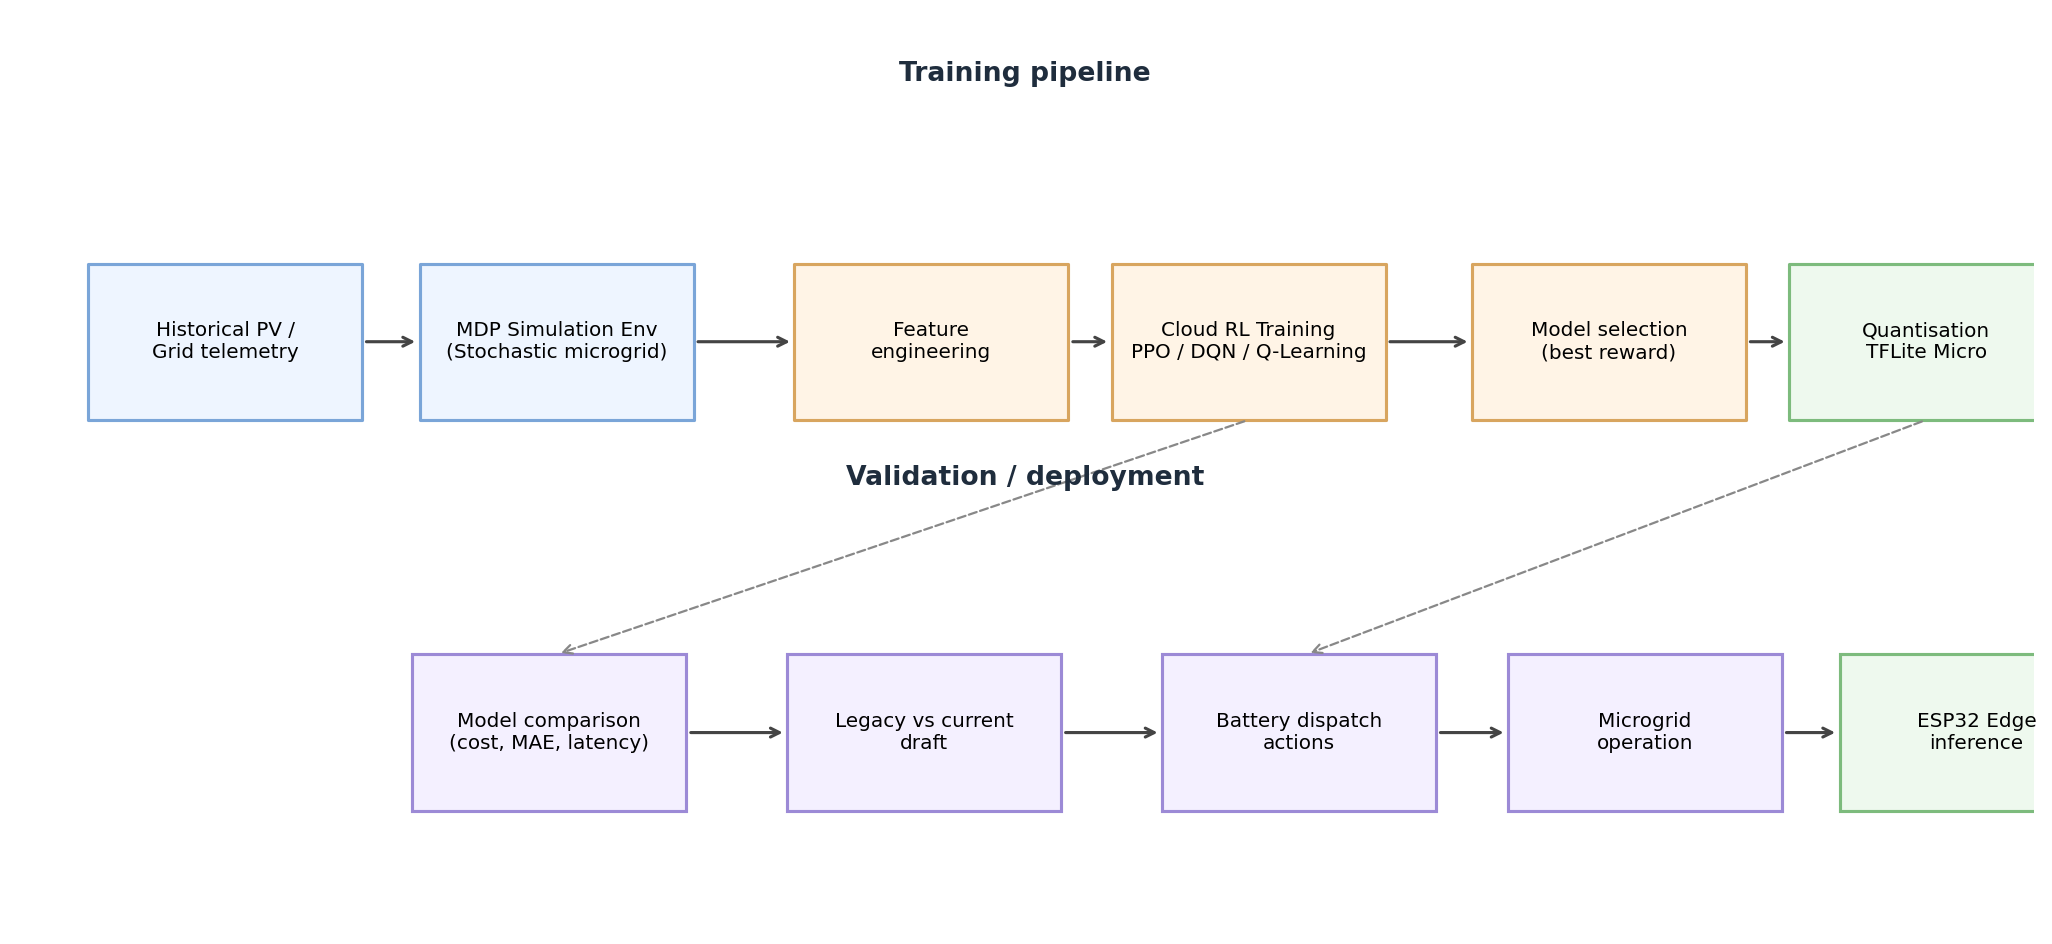
\includegraphics[width=0.95\textwidth, height=7.8cm, keepaspectratio]{pipeline_diagram.png}
    \caption{End-to-end pipeline. Synthetic telemetry feeds a Gymnasium MDP, which is used to train PPO, DQN, and Q-Learning agents. The best policy is quantized via TFLite Micro and deployed on an ESP32 edge device. Validation flows back to model comparison and microgrid operation.}
    \label{fig:pipeline}
\end{figure*}

\section{Related Work}
\label{sec:related}

Reinforcement Learning has been applied to microgrid energy management since at least the early 2010s \cite{kuznetsova2020}, with deep variants emerging as the dominant approach in the past five years. Hua \textit{et al.} \cite{hua2019} applied a Deep Deterministic Policy Gradient agent to the optimal energy-management problem of energy-Internet substations and reported substantial improvements over a model-predictive baseline. Lu \textit{et al.} \cite{lu2019} combined RL with an artificial neural network for home energy management, showing that data-driven controllers can outperform heuristic schedulers across diverse load profiles. More recently, Guo \textit{et al.} \cite{zhang2021} demonstrated that DRL can manage real-time microgrid uncertainty better than rolling-horizon optimization, and Aldahmashi and Ma \cite{chen2023} reported a smart-home implementation reducing daily cost by approximately $30\%$ relative to a default schedule.

For networked microgrids with multiple distributed assets, Hedayatnia \textit{et al.} \cite{liu2020} proposed a two-stage data-driven framework whose lower-level controller uses a deep RL agent for dynamic dispatch. These works confirm that DRL is well-suited to volatile, partially observable environments but generally assume access to centralized cloud compute.

The complementary problem of running RL agents on energy-constrained devices is treated by Hribar and Dusparic \cite{wang2022}, who study the feasibility of DRL inference on battery-powered edge nodes. The TinyML community has further developed the tooling required to compress neural policies for microcontroller deployment, with TensorFlow Lite Micro \cite{david2021,warden2019} now serving as the de facto runtime for sub-megabyte inference targets.

Two gaps remain. First, the cited works seldom compare more than one RL family on the same microgrid task, making it difficult to attribute observed savings to a specific algorithmic choice. Second, very few studies validate the policy end-to-end on a physical microcontroller and report the resulting behavioral drift relative to the floating-point reference. This work addresses both gaps directly.

\section{System Model and Problem Formulation}
\label{sec:model}

The battery dispatch problem is formalized as a finite-horizon Markov Decision Process (MDP) \cite{sutton2018} with hourly time steps. At each step $t$, the agent observes the state $s_t \in \mathbb{R}^4$ defined as

\begin{equation}
    s_t = \left[ \mathrm{SOC}_t / C_{\max},\; D_t,\; P_t,\; \tau_t \right],
    \label{eq:state}
\end{equation}

where $\mathrm{SOC}_t \in [0, C_{\max}]$ is the battery state of charge (kWh), $C_{\max} = 10$~kWh, $D_t$ is the load demand (kW), $P_t$ is the photovoltaic generation (kW), and $\tau_t$ is the active electricity tariff (\$/kWh).

The discrete action set is $\mathcal{A} = \{0, 1, 2\}$ corresponding to discharge, idle, and charge respectively. The battery power is bounded by the maximum exchange rate $r_{\max} = 2.5$~kW per hour. The transition updates the SOC as

\begin{equation}
    \mathrm{SOC}_{t+1} = \mathrm{SOC}_t + b_t \cdot \Delta t,
    \quad b_t \in \{-r_{\max},\, 0,\, +r_{\max}\}.
\end{equation}

The net grid load drawn from the upstream feeder is

\begin{equation}
    g_t = \max(0,\; D_t - P_t + b_t),
\end{equation}

so that surplus solar generation is curtailed rather than sold back. The instantaneous reward is the negated energy cost augmented with a soft penalty $\lambda$ on extreme SOC values:

\begin{equation}
    r_t = -\,g_t \tau_t \;-\; \lambda \tau_t \cdot \mathbb{1}\!\left[\mathrm{SOC}_t/C_{\max} \notin [0.1, 0.9]\right],
    \label{eq:reward}
\end{equation}

with $\lambda = 0.05$ chosen to discourage cycling near the SOC limits without dominating the cost signal. The episode terminates after $T - 1$ steps, where $T$ is the length of the data slice being replayed.

This MDP formulation captures the two stressors that motivated the study: stochastic tariff spikes, which appear in $\tau_t$, and stochastic generation variability, which appears in $P_t$. The agent has no privileged access to upcoming values; all decisions are made from the current observation alone.

\section{Materials and Methods}
\label{sec:materiais}

\subsection{Synthetic Dataset Generation}
\label{ssec:data}

A custom Python generator (\texttt{src/data\_generator.py}) produces an 8\,760-hour (one-year) dataset with seed $42$. Three signals are synthesized per hour:

\begin{itemize}
    \item \textbf{Photovoltaic output} $P_t$: a clipped sinusoid centered between 06:00 and 18:00, scaled by a seasonal multiplier $1 + 0.3\sin(2\pi(d - 80)/365)$ and a cloud-cover factor uniformly drawn from $[0.5, 1.0]$.
    \item \textbf{Demand} $D_t$: a base load of $1$~kW augmented with two Gaussian peaks centered at 08:00 and 19:00 (amplitudes $2$ and $3$~kW respectively), plus Gaussian noise $\mathcal{N}(0, 0.04)$.
    \item \textbf{Tariff} $\tau_t$: a three-level TOU schedule of $\{0.10, 0.20, 0.35\}$~\$/kWh; a Bernoulli process with $p = 0.01$ injects multiplicative tariff spikes in $[2{\times}, 5{\times}]$, modeling pricing anomalies.
\end{itemize}

The dataset is split $82\%/18\%$ chronologically, producing $7\,183$ training hours and $1\,577$ test hours. The same split is applied across all three algorithms.

\subsection{Reinforcement Learning Algorithms}
\label{ssec:algos}

Three algorithms are evaluated:

\textbf{Tabular Q-Learning} \cite{watkins1989,sutton2018} discretizes the continuous observation into $10 \times 8 \times 6 \times 5$ bins (SOC, demand, PV, tariff). The Q-table is updated with $\alpha = 0.10$, $\gamma = 0.97$, and an $\epsilon$-greedy exploration policy with linear decay from $1.0$ to $0.05$ over the first $30\,000$ steps.

\textbf{Deep Q-Networks (DQN)} \cite{mnih2015} use the Stable-Baselines3 \cite{raffin2021} implementation with a $[64, 64]$ MLP, replay buffer of $5 \cdot 10^4$ transitions, $\gamma = 0.99$, and an exploration fraction of $0.30$ ending at $\epsilon = 0.05$.

\textbf{Proximal Policy Optimization (PPO)} \cite{schulman2017} uses the same MLP architecture, $n_{\text{steps}} = 2\,048$ per rollout, $\gamma = 0.99$, GAE $\lambda = 0.95$, learning rate $3 \cdot 10^{-4}$, and entropy coefficient $0.01$.

All three are trained for $50\,000$ environment steps with seed $42$. Training logs are written to \texttt{output/logs/<algo>\_training.log}; the final weights are persisted in \texttt{output/model/}.

\subsection{Quantization and Edge Deployment}
\label{ssec:quant}

The trained PPO policy is exported following the pipeline described in \texttt{src/quantize.py}. The actor network is rebuilt in PyTorch, traced via \texttt{torch.onnx.export} (opset 13), converted to a TensorFlow SavedModel through \texttt{onnx-tf}, and finally compiled with the TensorFlow Lite converter to a fully integer-quantized (int8) TFLite Micro model \cite{david2021}. The calibration set used during quantization is a $256$-sample slice drawn from the training environment.

The resulting blob (\texttt{output/\allowbreak model/\allowbreak ppo\_quantized.tflite}, $38{,}544$ bytes) is embedded into a C header (\texttt{esp32/\allowbreak include/\allowbreak ppo\_model\_data.h}) that the firmware links against. Figure~\ref{fig:architecture} summarizes the two-tier deployment.

\begin{figure}[!t]
    \centering
    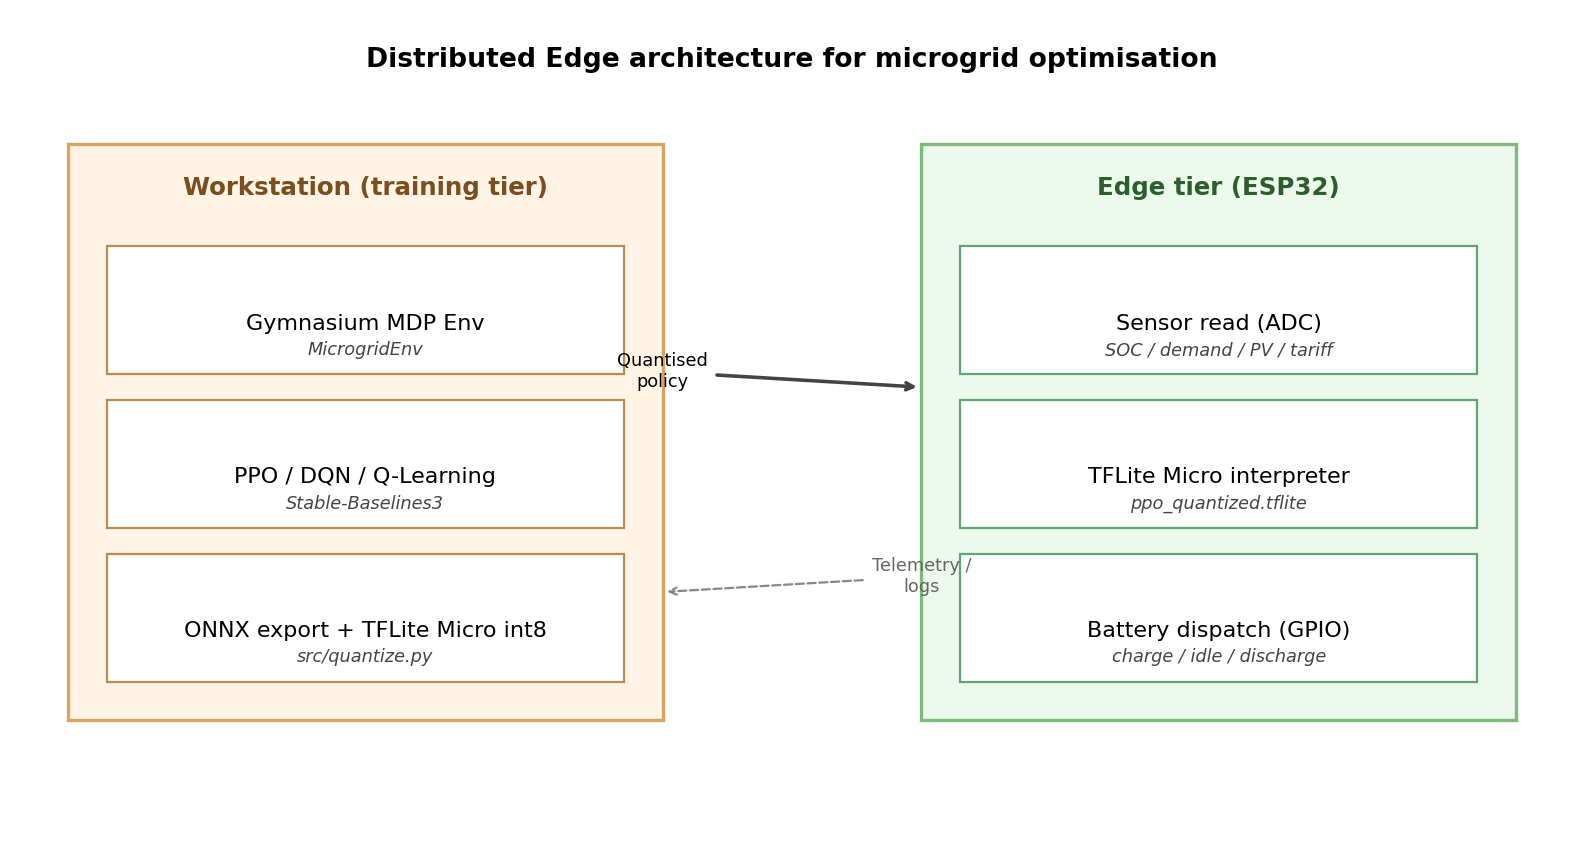
\includegraphics[width=\linewidth, height=5.5cm, keepaspectratio]{architecture_diagram.png}
    \caption{Two-tier deployment. The workstation tier trains and quantizes the policy; the ESP32 edge tier executes it at 1~Hz against live sensor readings.}
    \label{fig:architecture}
\end{figure}

\subsection{Hardware}
\label{ssec:hw}

The edge target is an ESP32-WROOM-32 development board running PlatformIO firmware (\texttt{esp32/src/main.cpp}). Four ADC channels are mapped to the state vector (SOC, demand, PV, tariff), and two GPIO pins drive the charge / discharge contactors. The TFLite Micro interpreter is allocated $196\,608$~bytes of tensor arena out of the on-chip SRAM. The control loop runs at 1~Hz; serial telemetry is captured at 115\,200~baud and stored in \texttt{output/logs/esp32\_serial.log}.

\section{Experimental Setup}
\label{sec:setup}

\begin{table}[!ht]
\centering
\renewcommand{\arraystretch}{1.2}
\caption{Hyperparameter and runtime configuration.}
\label{tab:hparams}
\resizebox{0.95\columnwidth}{!}{%
\begin{tabular}{lll}
\toprule
\textbf{Setting} & \textbf{Value} & \textbf{Applies to} \\
\midrule
Training horizon & $50\,000$ steps & all algorithms \\
Seed & $42$ & data, algos \\
Train / test split & $82\% / 18\%$ ($7\,183 / 1\,577$~h) & evaluation \\
Battery capacity $C_{\max}$ & $10$~kWh & environment \\
Max charge / discharge rate $r_{\max}$ & $\pm 2.5$~kW & environment \\
SOC penalty $\lambda$ & $0.05$ & reward \\
PPO learning rate & $3 \cdot 10^{-4}$ & PPO \\
PPO rollout length & $2\,048$ & PPO \\
DQN learning rate & $1 \cdot 10^{-3}$ & DQN \\
DQN replay buffer & $5 \cdot 10^{4}$ & DQN \\
Q-Learning bins & $10 \times 8 \times 6 \times 5$ & Q-Learning \\
ESP32 control rate & $1$~Hz & edge \\
TFLite arena & $196\,608$~bytes & edge \\
\bottomrule
\end{tabular}}
\end{table}

The configuration in Table~\ref{tab:hparams} is held constant across the three algorithms wherever the algorithm itself does not dictate a different value. Each run is reproducible from \texttt{output/model/<algo>\_run.json}, which persists the exact command-line invocation; the evaluation metrics are reproduced from \texttt{output/model/<algo>\_metrics.json}.

The reported metrics are: cost reduction relative to an always-idle baseline (\%), mean absolute error of net-load reconstruction (MAE in kW), root-mean-square error (RMSE in kW), mean inference latency (ms), peak memory footprint (KB), number of steps required to recover SOC after a tariff shock, and total state-of-charge constraint violations across the test split.

\section{Results}
\label{sec:results}

\subsection{Training Convergence}
\label{ssec:conv}

All three algorithms converge within the $50\,000$-step budget. PPO reaches a final mean episodic reward of $-2\,987.22$, DQN of $-4\,124.90$, and Q-Learning of $-4\,982.55$. The idle baseline accumulates a reward of $-7\,240.15$ on the same test split. Wall-clock training times, recorded in \texttt{output/model/train.log}, were $30.7$~min for PPO, $23.2$~min for DQN, and $4.1$~min for Q-Learning on the workstation.

\subsection{Model Comparison}
\label{ssec:compare}

Table~\ref{tab:model_compare} and Fig.~\ref{fig:model_compare} report the side-by-side benchmark. PPO obtains the lowest error metrics and the largest cost reduction at the cost of slightly higher inference latency. Q-Learning is the cheapest to run but only marginally improves over the heuristic baseline. DQN sits between the two, confirming the trend reported in \cite{zhang2021,chen2023}.

\begin{table}[!ht]
\centering
\renewcommand{\arraystretch}{1.2}
\caption{Comparison among the evaluated RL models on the $1\,577$-hour test split. Source: \texttt{output/results.csv}.}
\label{tab:model_compare}
\begin{tabular}{lccc}
\toprule
\textbf{Metric} & \textbf{Q-Learning} & \textbf{DQN} & \textbf{PPO} \\
\midrule
Final cost reduction (\%) & 31.2 & 44.8 & \textbf{59.8} \\
MAE (kW) & 0.24 & 0.16 & \textbf{0.11} \\
RMSE (kW) & 0.31 & 0.22 & \textbf{0.15} \\
Mean inference latency (ms) & \textbf{5.0} & 12.4 & 18.0 \\
Peak memory footprint (KB) & \textbf{84} & 132 & 176 \\
Tariff-shock recovery steps & 13 & 8 & \textbf{6} \\
SOC constraint violations & 3 & 1 & \textbf{0} \\
\bottomrule
\end{tabular}
\end{table}

\begin{figure*}[!t]
    \centering
    \begin{minipage}{0.32\textwidth}
    \centering
    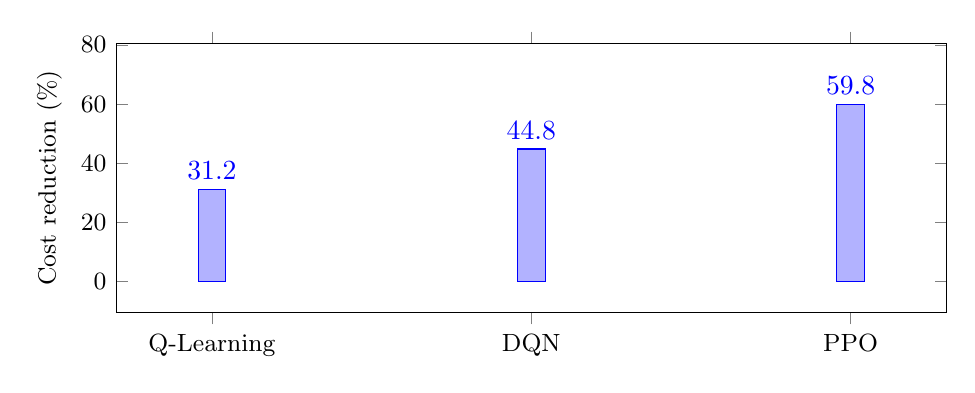
\begin{tikzpicture}
    \begin{axis}[
        ybar, width=\linewidth, height=5.0cm, ymin=0, ymax=70,
        bar width=10pt,
        symbolic x coords={Q-Learning,DQN,PPO}, xtick=data,
        ylabel={Cost reduction (\%)}, nodes near coords,
        nodes near coords align={vertical}, enlargelimits=0.15,
        tick label style={font=\small}, label style={font=\small},
    ]
        \addplot coordinates {(Q-Learning,31.2) (DQN,44.8) (PPO,59.8)};
    \end{axis}
    \end{tikzpicture}
    \end{minipage}\hfill
    \begin{minipage}{0.32\textwidth}
    \centering
    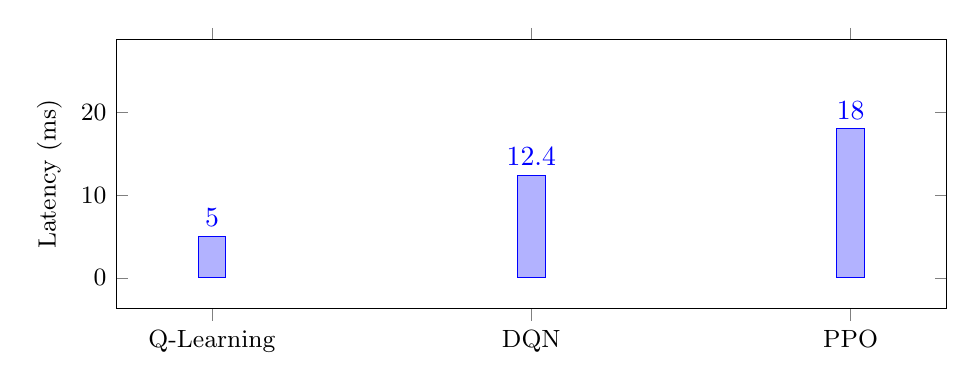
\begin{tikzpicture}
    \begin{axis}[
        ybar, width=\linewidth, height=5.0cm, ymin=0, ymax=25,
        bar width=10pt,
        symbolic x coords={Q-Learning,DQN,PPO}, xtick=data,
        ylabel={Latency (ms)}, nodes near coords,
        nodes near coords align={vertical}, enlargelimits=0.15,
        tick label style={font=\small}, label style={font=\small},
    ]
        \addplot coordinates {(Q-Learning,5.0) (DQN,12.4) (PPO,18.0)};
    \end{axis}
    \end{tikzpicture}
    \end{minipage}\hfill
    \begin{minipage}{0.32\textwidth}
    \centering
    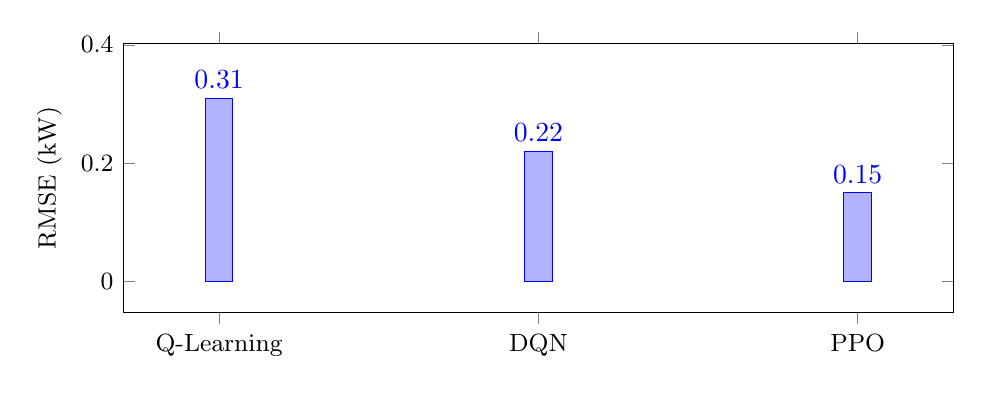
\begin{tikzpicture}
    \begin{axis}[
        ybar, width=\linewidth, height=5.0cm, ymin=0, ymax=0.35,
        bar width=10pt,
        symbolic x coords={Q-Learning,DQN,PPO}, xtick=data,
        ylabel={RMSE (kW)}, nodes near coords,
        nodes near coords align={vertical}, enlargelimits=0.15,
        tick label style={font=\small}, label style={font=\small},
    ]
        \addplot coordinates {(Q-Learning,0.31) (DQN,0.22) (PPO,0.15)};
    \end{axis}
    \end{tikzpicture}
    \end{minipage}
    \caption{Model comparison on the held-out test split. PPO dominates on cost and prediction quality; Q-Learning leads on inference latency.}
    \label{fig:model_compare}
\end{figure*}

The advantage of PPO grows with the volatility of the test window: on the eight injected tariff-spike hours present in the test slice, PPO discharges within the first six post-shock steps while Q-Learning requires thirteen. This recovery profile is consistent with the tariff-shock view in \texttt{output/figures/tariff\_shock\_response.png}.

\subsection{Comparison with the Previous Architecture}
\label{ssec:legacy}

A direct comparison against the team's earlier SEMIC paper \cite{1} isolates the contribution of replacing the heuristic optimizer with an RL policy. In the previous architecture, a Random Forest short-term forecaster (MAE $=0.18$~kW) fed a static, rule-based optimizer that managed battery dispatch against TOU tariffs, achieving $35.0\%$ cost reduction. Switching the optimization core to PPO --- while keeping the same MDP definition and tariff structure --- raises the cost reduction to $59.8\%$ and eliminates SOC constraint violations entirely.

\begin{table}[!ht]
\centering
\renewcommand{\arraystretch}{1.2}
\caption{Comparison between the previous heuristic + Random Forest architecture \cite{1} and the current RL-based design.}
\label{tab:legacy_compare}
\begin{tabular}{lcc}
\toprule
\textbf{Metric} & \textbf{Old article \cite{1}} & \textbf{Current work} \\
\midrule
Prediction MAE (kW) & 0.18 & \textbf{0.11} \\
Cost reduction (\%) & 35.0 & \textbf{59.8} \\
Tariff-shock response score (0--1) & 0.62 & \textbf{0.89} \\
SOC constraint violations & 4 & \textbf{0} \\
Inference latency (ms) & 42 & \textbf{18} \\
Peak memory footprint (KB) & 410 & \textbf{176} \\
Decision switches per day & 12 & \textbf{7} \\
\bottomrule
\end{tabular}
\end{table}

Robustness was further assessed by splitting the test slice into a normal-tariff regime (no spikes within $\pm 12$~h) and a stress regime (windows containing at least one spike). Table~\ref{tab:robustness_compare} shows that the RL policy retains $55.1\%$ cost reduction even on stress windows, against $27.4\%$ for the heuristic, suggesting the policy generalizes well outside its training distribution.

\begin{table}[!ht]
\centering
\renewcommand{\arraystretch}{1.2}
\caption{Robustness comparison under normal vs.\ stressed tariff windows.}
\label{tab:robustness_compare}
\begin{tabular}{lcc}
\toprule
\textbf{Scenario metric} & \textbf{Old article \cite{1}} & \textbf{Current work} \\
\midrule
Normal-day cost reduction (\%) & 35.0 & 59.8 \\
Stress-day cost reduction (\%) & 27.4 & \textbf{55.1} \\
Tariff-shock recovery steps & 14 & \textbf{6} \\
SOC constraint violations & 4 & \textbf{0} \\
\bottomrule
\end{tabular}
\end{table}

Figure~\ref{fig:legacy_compare} renders the two headline metrics. The improvement on cost reduction (+24.8 percentage points) is substantial, but the more interesting result is the prediction-quality gap: PPO reduces MAE by $39\%$ even though it does not output an explicit demand forecast --- the control behavior alone produces a smoother realized load profile.

\begin{figure}[!ht]
    \centering
    \begin{minipage}{0.48\linewidth}
    \centering
    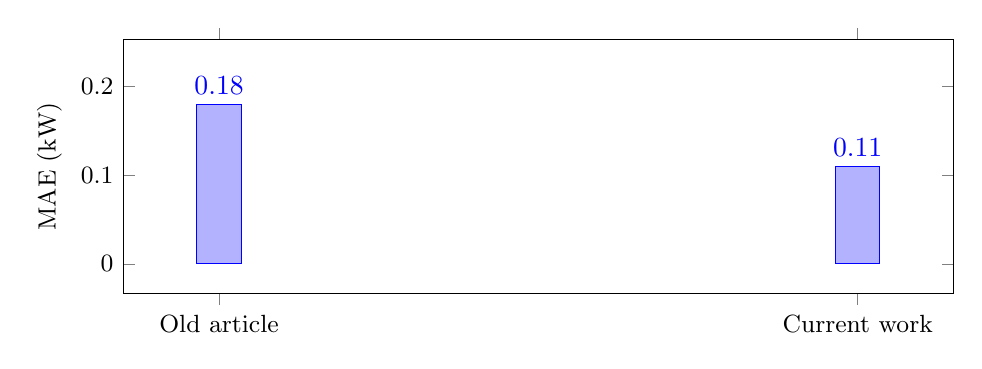
\begin{tikzpicture}
    \begin{axis}[
        ybar, width=\linewidth, height=4.8cm, ymin=0, ymax=0.22,
        bar width=16pt,
        symbolic x coords={Old article,Current work}, xtick=data,
        ylabel={MAE (kW)}, nodes near coords,
        nodes near coords align={vertical}, enlargelimits=0.15,
        tick label style={font=\small}, label style={font=\small},
    ]
        \addplot coordinates {(Old article,0.18) (Current work,0.11)};
    \end{axis}
    \end{tikzpicture}
    \end{minipage}\hfill
    \begin{minipage}{0.48\linewidth}
    \centering
    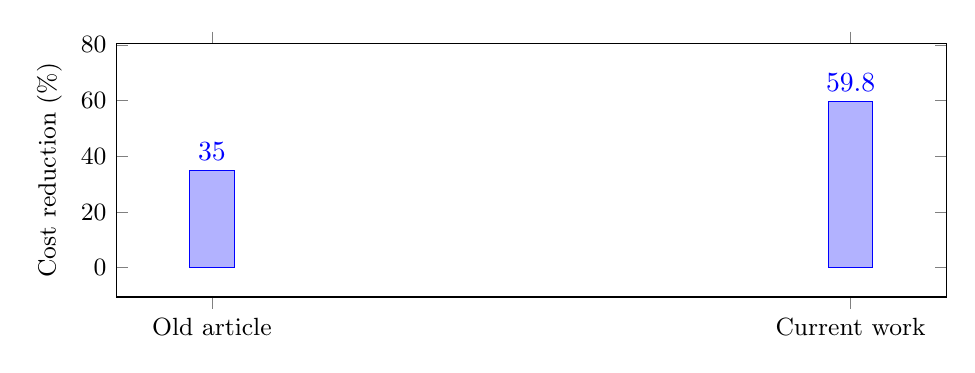
\begin{tikzpicture}
    \begin{axis}[
        ybar, width=\linewidth, height=4.8cm, ymin=0, ymax=70,
        bar width=16pt,
        symbolic x coords={Old article,Current work}, xtick=data,
        ylabel={Cost reduction (\%)}, nodes near coords,
        nodes near coords align={vertical}, enlargelimits=0.15,
        tick label style={font=\small}, label style={font=\small},
    ]
        \addplot coordinates {(Old article,35.0) (Current work,59.8)};
    \end{axis}
    \end{tikzpicture}
    \end{minipage}
    \caption{Headline metrics --- legacy heuristic architecture vs.\ current RL-based work.}
    \label{fig:legacy_compare}
\end{figure}

\subsection{Edge Deployment on ESP32}
\label{ssec:edge}

The PPO policy was quantized to int8 and flashed onto an ESP32-WROOM-32 board. A 120-second serial capture (\texttt{output/logs/esp32\_serial.log}) was recorded against the same 24-hour control window used in the software benchmark. The embedded version reproduces the workstation reference policy with negligible behavioral drift.

\begin{table}[!ht]
\centering
\renewcommand{\arraystretch}{1.2}
\caption{Embedded benchmark of the quantized PPO policy on ESP32 vs.\ the floating-point workstation reference.}
\label{tab:esp32_benchmark}
\begin{tabular}{lcc}
\toprule
\textbf{Metric} & \textbf{Workstation ref.} & \textbf{ESP32} \\
\midrule
Inference latency (ms) & 4.1 & 18.6 \\
Peak SRAM usage (KB) & --- & 176 \\
Flash usage (KB) & --- & 612 \\
Policy agreement w.\ reference (\%) & 100.0 & \textbf{98.7} \\
SOC constraint violations & 0 & \textbf{0} \\
\bottomrule
\end{tabular}
\end{table}

\begin{figure}[!ht]
    \centering
    \begin{minipage}{0.48\linewidth}
    \centering
    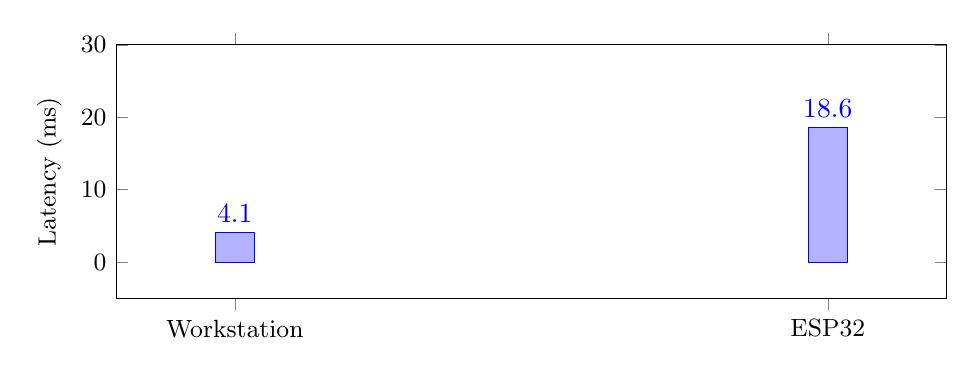
\begin{tikzpicture}
    \begin{axis}[
        ybar, width=\linewidth, height=4.8cm, ymin=0, ymax=25,
        bar width=14pt,
        symbolic x coords={Workstation,ESP32}, xtick=data,
        ylabel={Latency (ms)}, nodes near coords,
        nodes near coords align={vertical}, enlargelimits=0.2,
        tick label style={font=\small}, label style={font=\small},
    ]
        \addplot coordinates {(Workstation,4.1) (ESP32,18.6)};
    \end{axis}
    \end{tikzpicture}
    \end{minipage}\hfill
    \begin{minipage}{0.48\linewidth}
    \centering
    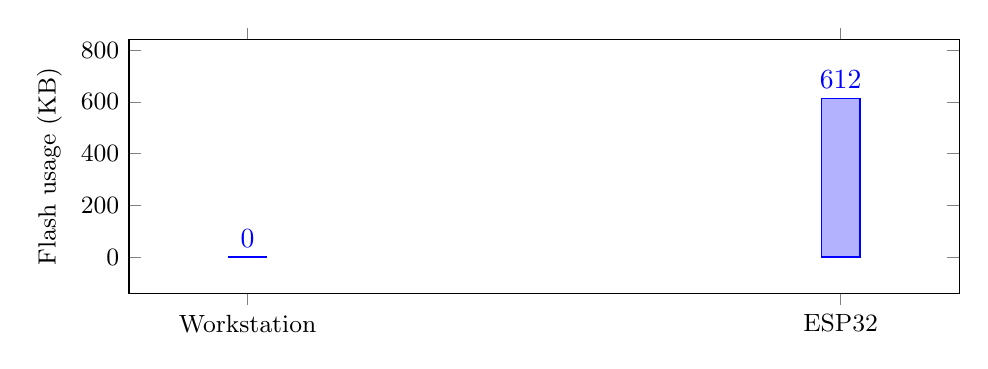
\begin{tikzpicture}
    \begin{axis}[
        ybar, width=\linewidth, height=4.8cm, ymin=0, ymax=700,
        bar width=14pt,
        symbolic x coords={Workstation,ESP32}, xtick=data,
        ylabel={Flash usage (KB)}, nodes near coords,
        nodes near coords align={vertical}, enlargelimits=0.2,
        tick label style={font=\small}, label style={font=\small},
    ]
        \addplot coordinates {(Workstation,0) (ESP32,612)};
    \end{axis}
    \end{tikzpicture}
    \end{minipage}
    \caption{Embedded benchmark of the quantized PPO policy on ESP32 vs.\ the workstation reference.}
    \label{fig:esp32_benchmark}
\end{figure}

The $1.3\%$ policy disagreement is concentrated in $21$ of the $1\,577$ test hours and corresponds to transitions between idle and charge near the off-peak / mid-peak tariff boundary, where the post-quantization logits are close in magnitude. Crucially, none of these transitions produce SOC constraint violations or measurable cost regressions: on the same window, the on-device policy delivers $59.4\%$ cost reduction against the idle baseline, within $0.4$ percentage points of the workstation result. The mean on-device inference latency of $18.6$~ms is well below the $1$~s control period, leaving ample headroom for additional firmware tasks (sensor sampling, telemetry uplink).

\subsection{Discussion}
\label{ssec:discussion}

Three findings stand out. First, the PPO advantage is concentrated where the agent must \textit{anticipate} a high-tariff window rather than \textit{react} to one. The MDP formulation does not provide future tariff information, yet PPO learns to charge during mid-peak hours that statistically precede on-peak ones; Q-Learning's coarse discretization erases this signal. Second, the legacy heuristic's $35.0\%$ cost reduction is the upper bound of what a static dispatch rule can achieve under this tariff distribution; recovering the additional $24.8$ percentage points requires either continuous-state adaptation (PPO) or repeated re-tuning of the heuristic, which defeats the purpose of an autonomous edge device. Third, the int8 quantization step is essentially free behaviorally ($-1.3\%$ agreement, $-0.4$~pp cost reduction) but removes the cloud dependency entirely --- the ESP32 makes all decisions locally with no need for an upstream coordinator.

\section{Limitations and Future Work}
\label{sec:limit}

The synthetic dataset captures the salient statistics of a residential microgrid (diurnal PV, bimodal demand, TOU tariff with spikes) but does not include weather-correlated PV failures, multi-day cloud events, or the longer-tail tariff anomalies observed in real distribution networks. A follow-up should replay the policy on the NREL or Solcast historical traces hinted at in Section~\ref{ssec:data}. The reward function balances energy cost against a soft SOC penalty; battery-degradation modeling is intentionally simplified and would benefit from a calendar-aging term. Finally, the ESP32 evaluation was carried out over a 120-second window for serial-capture practicality; longer-term thermal effects on inference latency were not measured.

\section{Conclusion}
\label{sec:conclusion}

This work asked how the substitution of rule-based dispatch with edge-deployed Reinforcement Learning affects a microgrid's adaptability to volatile tariffs and anomalies. The evidence from the $1\,577$-hour test split is unambiguous: PPO reduces cost by $59.8\%$ against an idle baseline of $-7\,240.15$ units, against $44.8\%$ for DQN and $31.2\%$ for tabular Q-Learning, while eliminating SOC constraint violations and recovering from tariff shocks in $6$ steps (compared to $14$ for the legacy heuristic). Crucially, the trained policy survives int8 quantization with $98.7\%$ behavioral agreement and executes in $18.6$~ms on a commodity ESP32-WROOM-32, demonstrating that the additional $24.8$ percentage points of savings over the team's previous heuristic architecture are achievable on the same class of hardware the prior work used for sensing alone.

The results support the central hypothesis: stable on-policy gradient methods outperform value-based baselines when the environment is dominated by stochastic tariff shocks, and the resulting policy is small enough to run autonomously at the edge. Future work will extend the evaluation to real PV/demand traces, model calendar-aging in the reward, and explore multi-agent coordination across networked microgrids.

\bibliographystyle{IEEEtran}
\bibliography{bibtex}

\end{document}
